% !TEX root = task-1-10-2.tex
% Editable task bank. Append new BankTask blocks at the end of the document.
\documentclass[12pt,a4paper]{article}
\usepackage{physics-textbook}
\usepackage{graphicx,needspace}
\usetikzlibrary{decorations.pathmorphing}
\newif\ifShowSolutions
\ifdefined\TutorEdition
  \ShowSolutionstrue
\else
  \ShowSolutionsfalse % Change to \ShowSolutionstrue to display solutions.
\fi
\newcounter{banktask}
\newsavebox{\BankTaskBox}
\newcommand{\BankTaskContent}[3]{%
  \noindent\textbf{\thebanktask.}\quad #2\par
  \ifShowSolutions
    \Needspace{50mm}% Keep the solution heading with its opening text or diagram.
    #3\par
    \ifdefined\TutorEdition
      \ifcsname TutorSource#1\endcsname
        \nopagebreak\smallskip{\small\csname TutorSource#1\endcsname\par}%
      \fi
    \fi
  \fi
}
\newcommand{\BankTask}[3]{%
  \refstepcounter{banktask}\par\medskip
  \sbox{\BankTaskBox}{\begin{minipage}{\linewidth}%
    \BankTaskContent{#1}{#2}{#3}\end{minipage}}%
  \ifdim\dimexpr\ht\BankTaskBox+\dp\BankTaskBox\relax>\dimexpr\textheight-20mm\relax
    \Needspace{35mm}\BankTaskContent{#1}{#2}{#3}%
  \else
    \Needspace{\dimexpr\ht\BankTaskBox+\dp\BankTaskBox\relax}%
    \noindent\usebox{\BankTaskBox}\par
  \fi
  \medskip
}
\begin{document}
\BookSubsection{1.10.2}{Сила тяжести}


% Source E11CE9: https://ege.fipi.ru/bank/questions.php?search=1&proj=BA1F39653304A5B041B656915DC36B38&qid=E11CE9
\BankTask{E11CE9}{
При помощи динамометра измеряют силу тяжести, действующую на пластину (см. рисунок). Динамометр проградуирован в ньютонах. Абсолютная погрешность прямого измерения силы динамометром равна цене деления. Какова сила тяжести, действующая на пластину, по показаниям динамометра?
\begin{center}
\par\begin{center}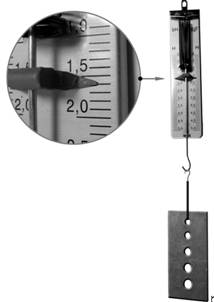
\includegraphics[width=.9\linewidth,height=.48\textheight,keepaspectratio]{_run/photos/4498756fd16b21134650ddd44db86764dbfe98f4a9c2e973429592f86033453e.png}\end{center}\par
\end{center}
}{
\smallskip\noindent\textbf{Решение от GPT}\par
Цена деления динамометра равна $(2{,}0-1{,}5)/5=0{,}1\,\text{Н}$. Указатель показывает $1{,}6\,\text{Н}$; это сила тяжести, уравновешенная силой упругости. С учётом погрешности $F_{\text{тяж}}=(1{,}6\pm0{,}1)\,\text{Н}$.
}

\end{document}
